\section{Proof of Concept: Neural Network codec for Video conferencing}

Google Colab is a product from Google Research that allows us to run python code through a Jupyter notebook-based User Interface. 
It hosts a customized Jupyter notebook service, set up on the cloud, enabling easier access for machine learners, data analysts, and academicians. The best part about Google Colab is its dynamic and free access to GPU and CPU compute on the cloud. Furthermore, saving the notebooks on Google Drive facilitates sharing and easy collaboration. It also supports loading python notebooks from GitHub gists. 
Google Colab instances also have a wide variety of pre-installed libraries.

The only bottleneck is that resources are offered virtually over the cloud, which can get reset or deleted if a higher priority task demands for the compute. Google also restricts the lifetime of an instance to prevent abuse.

OpenCV is a library used for image capture, processing, and knowledge extraction. For the proof of concept, OpenCV was used to capture an image and video from the user's webcam. This image is then stored, and also converted into an array, to feed to the pre-trained First Order Motion Model 
neural network.

The First Order Motion Model Neural Network functions by identifying the objects in the source image and driving video. It then animates the object depicted in the source image based on the motion of a similar object in the driving video. This approach is self-supervised, and mainly functions by 
observing frame pairs extracted from the driving video, relatively displacing the key points of the image to match that of the driving video.

\begin{figure}[h]
    \begin{center}
        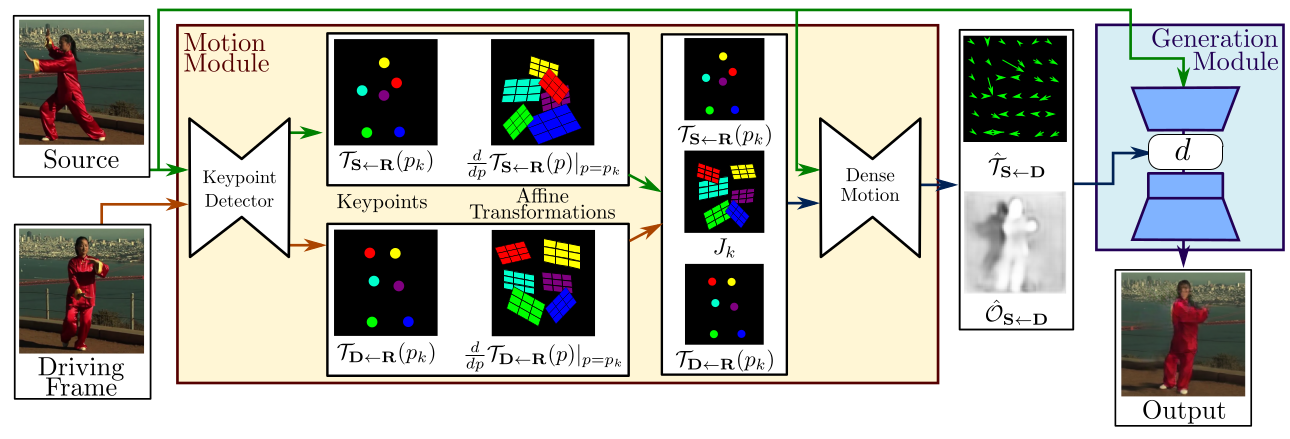
\includegraphics[width=15cm]{FOMM-overview-approach.png}
    \end{center}
    \caption{An overview of the First Order Motion Model.}
    \label{fig:FOMMoverview}
\end{figure}

As can be seen in figure \ref{fig:FOMMoverview}, the neural network has two major components, the motion module, and the generation module. 
The data transferred between both modules consists of a set of jacobian matrices which contain the displacement of the main key points. 
Our approach transfers a compressed version of these jacobian matrices over the internet, reducing the network overhead. It follows these basic steps: 

\begin{itemize}
    \item First record a video of the user as if they were using a video-conferencing application. 
    \item The first frame recorded by the webcam is used as the keyframe, which is fed as the source image to the First Order Motion Model.
    \item The remaining frames of the video are then sent as the driving video to the First Order Motion Model.
    \item The model then generates the jacobians and we measure the amount of data being transferred.
    \item The jacobians are then used to generate a final image, which gets viewed at the other side of the video conferencing conversation.
\end{itemize}